\chapter{Preliminary Study}

\minitoc

This chapter is ment to outline the preliminary study of our project. This includes what our technologies aims to achive and how we will use them to achive this. Beyond this, the chapter will show the methology the team chose too use and why this was a natural choce to go with. Research in software testing methods will be included and the best fit for this project. Since this is a prototype project, a considrible time is put into this part of the project, to assure the team makes good choices when it comes to thecnologies to use.

\clearpage

\section{Concept}
The efficiency of the power user can always be increased. And one way of achieving this efficency boost is through adding new functionality, but for bigger systems, this functionality adding can prove to be troublesome. Switching between the mouse and the keyboard can add up to be timeconsuming in the long run, and also inefficient. With an envinonment where the user then instead can construct their own functionality, and keep their hands on the keyboard, can add tremendous value to the user experience. This can be made possible with a scripting environment, where the user themselves will be given the oppurtunity to work through a console on their graphical user interface. This can release them from the mouse and let them work more efficiently on the tasks at hand. 

\section{Similar solutions}
In this section, we will discuss similar solutions and their relevance to our project.

\begin{center}
\begin{tabularx}{\textwidth}{ l X }
\hline
\textbf{Product} & Counter-Strike \\ \hline
\textbf{Concept} & This game features a console that offers a wide variety of commands, including:
- Changing the game options
- Altering the game world
- Player actions and cheats
- Multiplayer communication and administration \\ \hline
\textbf{Intended use} & In a game, this functionality eases development and debugging, as well as increasing the moddability and long-term value for players. \\ \hline
\textbf{Similar products} & Similar consoles also exist in other games, such as Carmageddon TDR 2000. \\ \hline
\textbf{Relationship to our project} & Like our project, the Counter-Strike console allows for using a DSL to work with objects in its given domain. It shows that the console can be a powerful tool that comes at a relatively small development cost compared to designing a GUI with a similar feature set. \\ \hline
\end{tabularx}
\captionof{table}{Counter-Strike Console}\label{tab:csc}
\end{center}

\begin{center}
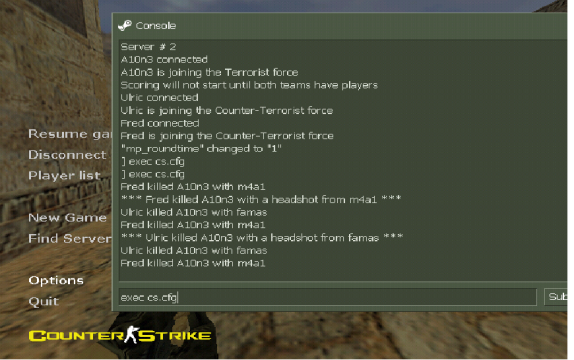
\includegraphics[width = 0.8\textwidth]{image/counterstrike.png}
\captionof{figure}{Counter-Strike Console}\label{cscimage}%
\end{center}

\begin{center}
\begin{tabularx}{\textwidth}{ l X }
\hline
\textbf{Product} & Blender \\ \hline
\textbf{Concept} & This 3D modelling software features a Python console with access to the model data, animation data, etc. It is also common to extend the program using custom Python scripts. \\ \hline
\textbf{Intended use} & In a creative suite, this type of functionality can be used to perform operations that are not directly supported in the user interface. It is particularly useful for programmatically executing repetitive tasks that can be automatized. \\ \hline
\textbf{Similar products} & Similar solutions also exist in other creative tools, including a Python console in GIMP and Nyquist prompt in Audacity. \\ \hline
\textbf{Relationship to our project} & The Blender console exposes the underlying data structures to the user via an already widespread, powerful scripting language. This enables the users themselves to expand upon the functionality of the program and perform operations that would be prohibitively time-consuming to execute manually. \\ \hline
\end{tabularx}
\captionof{table}{Blender Console}\label{tab:blenderc}
\end{center}

\begin{center}
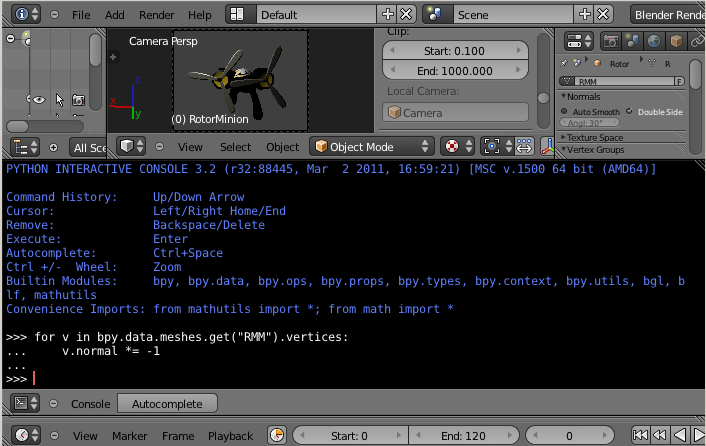
\includegraphics[width = 0.8\textwidth]{image/blender.png}
\captionof{figure}{Blender Console}\label{blendercimage}%
\end{center}

\begin{center}
\begin{tabularx}{\textwidth}{ l X }
\hline
\textbf{Product} & Firefox \\ \hline
\textbf{Concept} & This web browser features a Web Console where it is possible to execute JavaScript commands with access to the objects on the current page. \\ \hline
\textbf{Intended use} & In a web browser, this is useful for web development, prototyping and debugging for websites that use JavaScript. \\ \hline
\textbf{Similar products} & Similar features also exist in a few other browsers, such as Google Chrome. \\ \hline
\textbf{Relationship to our project} & Like our project, the Firefox Web Console offers access to the objects on a web page. It is possible for us to use the same principle, but for features that are useful for the end user and not just the developer. \\ \hline
\end{tabularx}
\captionof{table}{Firefox Web Console}\label{tab:firefoxc}
\end{center}

\begin{center}
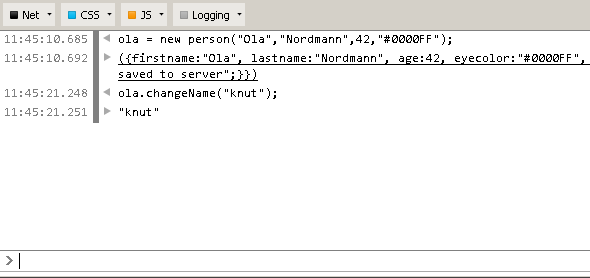
\includegraphics[width = 0.8\textwidth]{image/firefox.png}
\captionof{figure}{Firefox Web console}\label{firefoxcimage}%
\end{center}


\begin{center}
\begin{tabularx}{\textwidth}{ l X }
\hline
\textbf{Product} & try.mongodb.org \\ \hline
\textbf{Concept} & This database website features a console where the user can execute commands on a dummy database. \\ \hline
\textbf{Intended use} & On this website, the console serves as an educational and demonstrational tool for people who don't want to invest too much time in learning about the database system. \\ \hline
\textbf{Similar products} & Comparable consoles also exist to allow the user to execute arbitrary queries in database administration tools such as PHPMyAdmin. \\ \hline
\textbf{Relationship to our project} & This console allows the user to execute queries directly on a database, and interestingly it allows input of objects with arbitrary structure. We will require persistent storage of our objects on a server, so this technology may be relevant. \\ \hline
\end{tabularx}
\captionof{table}{MongoDB Console}\label{tab:mongodbc}
\end{center}

\begin{center}
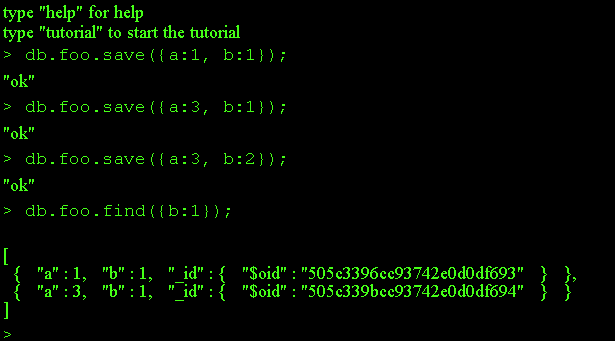
\includegraphics[width = 0.8\textwidth]{image/mongodb.png}
\captionof{figure}{MongoDB Console}\label{mongodbcimage}%
\end{center}


\begin{center}
\begin{tabularx}{\textwidth}{ l X }
\hline
\textbf{Product} & web-console.org \\ \hline
\textbf{Concept} & This project provides shell access to a server through the browser window over HTTP with support for real-time communication. \\ \hline
\textbf{Intended use} & This system is intended to be used for server administration purposes when HTTP may be the only feasible method of connection. \\ \hline
\textbf{Similar products} & Similar solutions include access to unix Shells via VPN. \\ \hline
\textbf{Relationship to our project} & If, in our project, the server is designed to support user input using a DSL in a terminal window, then a solution like this one may provide the necessary functionality to embed a useful console into a Web UI. \\ \hline
\end{tabularx}
\captionof{table}{Web-Console}\label{tab:webconsolec}
\end{center}

\begin{center}
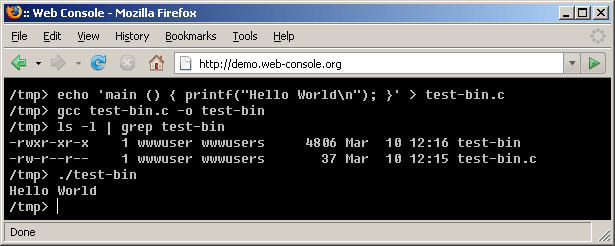
\includegraphics[width = 0.8\textwidth]{image/webconsole.png}
\captionof{figure}{Web- Console}\label{webconsolecimage}%
\end{center}

These products serve to illustrate that consoles are still applicable for purposes including software development, debugging, learning, extendability and where there is a high demand for flexibility. They can enhance productivity and provide features that would be prohibitively complex or expensive to implement in a graphical user interface. They also show that consoles do exist on the web, and that this is a field that is worth closer examination.


\section{Development language and technologies}
\subsection{Collaboration}

\subsubsection{Redmine}

\begin{wrapfigure}{r}{.25\textwidth}
\vspace{-30pt}
\centering

\includegraphics[width = .30\textwidth]{image/redmine-logo.pdf}
\end{wrapfigure}

Redmine is an online project management tool. It is an open source, cross-platform application. If offers role based access control, issue tracking system, Gantt chart display and browsing source code saved on git. We use this application for project planning and creating, assigning and logging issues. It can also be used as an alternative source code browser with its own automatically replicated copy of github repository. Information stored in the system is very important, so we set up automatic backup of the database to our git repository.
\footnote{http://www.redmine.org/projects/redmine/wiki}

\subsubsection{Google Calendar}

\begin{wrapfigure}{r}{.25\textwidth}
\vspace{-30pt}
\centering
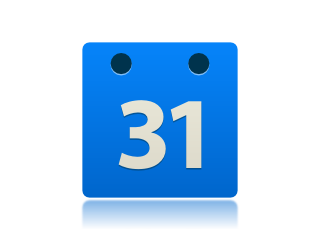
\includegraphics[width = .20\textwidth]{image/calendar-logo.png}
\end{wrapfigure}

Google Calendar is online time management tool, which enables users to create events in shared calendars. It is also possible to invite people to attend an event. We use it for planning the meetings, and put in important lectures and deadlines. Shared calendar is administered by team members. It will let the members use their favourite mail, whilest still receaving invitations to planned meetings.
\footnote{https://www.google.com/calendar}

Our group Google Calendar is available on page:
https://www.google.com/calendar/embed?src=6j792hr87jahd4vpnj636h1080%40group.calendar.google.com

\subsubsection{Google Groups}

\begin{wrapfigure}{r}{.25\textwidth}
\vspace{-30pt}
\centering

\includegraphics[width = .20\textwidth]{image/groups-logo.png}
\end{wrapfigure}

Google Groups is online communication tool. It offers group management and communication through web interface and email. We use it as a mailing list tool. Contact person publishes important news and information. Meeting dates and notes are distributed to all members of group. Customer and advisor can send emails directly to group email address, so that if contact person is not available at the moment, anyone from group can answer.

Our Google Group mailing list address is: ntnu-netlight-project@googlegroups.com
\footnote{https://groups.google.com/googlegroups/overview.html}

\subsubsection{Google Drive}

\begin{wrapfigure}{r}{.25\textwidth}
\vspace{-30pt}
\centering

\includegraphics[width = .20\textwidth]{image/drive-logo.jpg}
\end{wrapfigure}

A file storage and synchronization service. Google Drive is the home of Google Docs, which is a set of applications such as document editing, spreadsheet, powerpoint, etc. We use these applications to easy share all documents between all the members of our project. It lets us edit and work with the same documents separately at the same time, and keeps a safe backup in the Google Cloud of our files if some computers where to break down.
\footnote{http://en.wikipedia.org/wiki/Google\_Drive}


\subsubsection{Skype}

\begin{wrapfigure}{r}{.25\textwidth}
\vspace{-30pt}
\centering

\includegraphics[width = .20\textwidth]{image/skype-logo.png}
\end{wrapfigure}

A free P2P/client-server communication program. It lets the users communicate with each other through voice, video, instant messaging and file transferring. The users needs a Skype account to reach other Skype users. This program is a VoIP service which lets us communicate without any extra cost if connected to a network. We mainly use Skype for discussions when the group is not gathered, this also gives us a transcript of what was discussed. All the members possesed a skype account, which made it easy to set up a project group.
\footnote{http://en.wikipedia.org/wiki/Skype}

\subsubsection{GitHub} \label{GitHub}

\begin{wrapfigure}{r}{.25\textwidth}
\vspace{-30pt}
\centering

\includegraphics[width = .20\textwidth]{image/github-logo.png}
\end{wrapfigure}

Web-based hosting service for software development. It uses the Git revision control system. Git focus on speed, and gives the user full revision tracking. GitHub uses this to present different functionalities to the users, such as setting up repositories, forking repositories, writing wikis and setting up web pages for the repositories. This integrates well with the shared code and report writing.
\footnote{http://en.wikipedia.org/wiki/GitHub}
\footnote{http://en.wikipedia.org/wiki/Git\_\(software\)}

\subsubsection{LaTeX}

\begin{wrapfigure}{r}{.25\textwidth}
\vspace{-30pt}
\centering
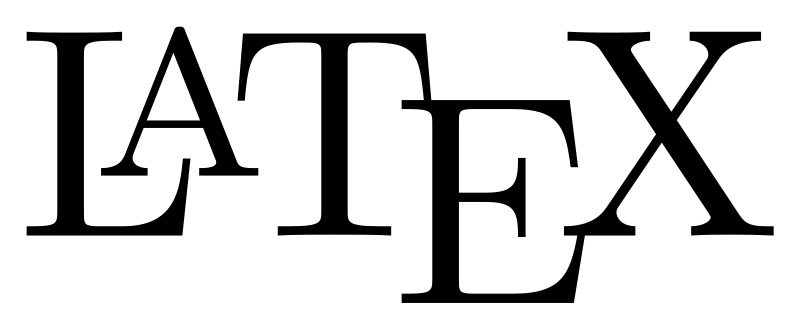
\includegraphics[width = .20\textwidth]{image/latex-logo.png}
\end{wrapfigure}

LaTex is a document markup language that uses the TeX typesetting program. The main focus of LaTex is to make authors able to focus on the content of what they are writing without worrying about its visual presentation. It is mainly used to transform XML- based documents to PDFs. LaTex is widely used in academia, to produce scientific reports, etc. This, and that the customer suggested it, made it a natural choice for the report. 

\subsection{Database}
For the system we need some kind of persistent storage, a database which all the clients can talk to to get the latest data in the system and to synchronise data from different clients. This database will be placed on a central server which all the clients can communicate with. For the database we are left with a decision between traditional SQL database or a so called NoSQL database. The differences are explained below.

\subsubsection*{NoSQL}
NoSQL databases are a group of new emerging types of databases that are defined by the fact that they are adressing some of the following points: being non-relational, distributed, open-source and horizontally scalable\cite{nosql}. NoSQL arose from the need to store large amount of data that do not necessarily follow the same schema, or share all the same attributes. One particular type of NoSQL databases that caught our attention early was the document NoSQL databases. The main characteristic of these databases is their schema- less structure. They also differ from SQL by generally not using a structured query language for data manipulation. They are easy to replicate and they offer simple APIs for the clients to communicate with. They are heavily customised for web- applications, and have gained much popularity in the modern web era. Most document NoSQL databases focus on quick replies to requests, as the queries operation is by far the most common in a typical web- application. Because they typically are distributed, NoSQL databases are able to store enormous amounts of data, and they are often used within Big Data\cite{bigdata} applications like Hadoop\cite{hadoop}, which recently has become a very popular subject within the computer science community. 
BASE \cite{pritchett} instead of ACID. 
Document NoSQL databases seemed like they would fit our project quite well.
\cite{nosql-databases, nosql-article}

\subsubsection*{SQL}
The traditional SQL databases is by far the most common way of storing data in the world today. They store data in columns and tables, and add relationships between these tables. As a result they are referred to as relational databases. They focus on query optimisation techniques and most of them use some kind of structured query language. Typically supports 4 basic operations which is select, update, delete and insert. SQL databases are schema defined and follows the ACID(atomicity, consistency, isolation, durability) principles.
\cite{ramakrishnan2003database}

\subsubsection{Database Alternatives}
Below, some of the database implementation available to us are discussed. We mainly investigated document NoSQL databases and regular SQL databses. The most appealing options are introduced below.

\subsubsection*{MongoDB}
MongoDB is a large scale, high availability, robust system. It is a document NoSQL system, so instead of storing the data in tables as you would in MySQL, the data is stored in a document based fashion through for instance JSON with dynamic schemas. This makes the DB easier scalable horizontally. But the mongoDB still possesses the some of the great properties from relational databases, such as indexes, dynamic queries and updates. With mongoDB it is easy to map objects to programming language data types, which makes the DB easy to work with. The embedded documents and arrays makes the join operations less importance, which result in the ability to make reads and writes faster. JavaScripts can also be included in the queries. This makes mongoDB an efficient and high speed data base for storing objects and fetching to a system. MongoDB also has its own access console, where you can use scripting with Javascript language. \cite{mongodb-intro}

\subsubsection*{CouchDB}
CouchDB stores the data in JSON documents(NoSQL) object-oriented, which can be accessed through HTTP. The data documents can be transformed and data fetched with JavaScript. CouchDB has a lot of built in features which makes web development with CouchDB easier. It scales well through replication and is a consistent system, where CouchDB prioritises the data of the user. CouchDB is multiversion concurrency control based, this is good for intense versioning, offline databases which resync later and master to master replication. The interface to the database is REST based, which is a useful feature when you are developing a web- application.
\cite{couchdb-about, couchdb-technical}

\subsubsection*{MySQL}
MySQL is the most popular database in the world of open databases. This is because of its high performance, reliability and ease of use, and should therefore be considered when the question comes to which database system to use. In opposition of the two database systems described above, MySQL is a relational database. This makes it more troublesome to work, with when it comes to JavaScript, than the other two. It is not as well integrated with JSON and will need parsing to be working with the clients. This alone is a hard negative towards MySQL.
\cite{mysql-about}


\subsubsection{Conclusion}
We decided to go for CouchDB in this project. We are working in a web domain, which CouchDB was designed for. While developing the console we will be working closely with JavaScript objects, and try to find ways of exposing these to the users. JavaScript objects are easily converted to JSON, the format used to store data in document NoSQL databases like MongoDB and CouchDB.  As we only have the need to store the actual objects and a limited amount of relations between them, using CouchDB will ease our work considerably, and allow us to do things which would not be possible with a regular SQL database. CouchDB imposes far less restrictions on how you store your data than traditional SQL does. As long as the data is represented in JSON, you can store pretty much store anything you like, even within the same database. This will give us great flexibility when it comes to adding information to specific objects, and also means that objects of the same type can contain different attributes without us needing to create a new schema or change anything in the database. It also gives the user great flexibility in the sense that they can add any information they would like to the different objects, and we the developers don't have to plan for it at all, the database does all this for us. As a result, instead of explicitly adding functionality, we can add restrictions to allow the user to add functionality within a certain scope. The fact that the customer suggested to us that we could use a NoSQL database, also tipped the scale in direction of the NoSQL alternatives. 

Relational databases is the traditional way to deploy databases and they are in widespread use. In many situations they are extremely useful. However relational databases requires you to model your data up front, before you save anything to the database. Failing to comply with these restrictions will lead to failure, and it is sometimes difficult to create this kind of model that actually fits real world data. Even though objects may share common attributes, there are bound to be some attributes that are different. This is difficult to plan for in advance, and its the main reason we will not be using a SQL database for this project. For the database, we originally chose to use MongoDB as our document NoSQL database. This was due to the fact that it was better documented and seemed better suited for the system as we originally planned it. Some of the features CouchDB offered wasn't thought of as necessary for the project at the time. During the implementation process we however came to the conclusion that CouchDb actually was a better fit. This was mostly due to its ability to act as an standalone system on a server without the need for other supporting server technologies like Node.js or ASP.NET. Also, the fact that it automaticly creates a RESTful API to access the database turned out to save us a lot of time. As a result of these discoveries we changed to CouchDb during the third sprint.


\subsection{Backend}
\subsubsection*{Node.js}
Node.js is a platform designed for server side applications. It is written in JavaScript using Google Chrome's JavaScript runtime called V8. The same runtime is used by the MongoDB database engine, so it shares some of its properties. It can be used for building fast and scalable network applications. Also it is very lightweight and efficient \cite{nodejs-about}.

\subsubsection*{ASP.NET}
ASP.NET is a part of the .NET Framework used for creating web applications and
services. The framework is language independent, so you can use any language
that .NET offers. It also allows programmers to use similar approach in web
applications as in desktop applications. On the other hand is not as lightweight as Node.js \cite{aspnet-about, palermo2010asp.net}.

\subsubsection*{PHP}
PHP is a acronym for Hypertext Preprocessor. It is a serverside programming language mainly used for web applications. PHP is easy to use and supports a lot of modules, platforms and database systems. One of the main disadvantages is, that is not as effective for web applications, because it is interpreted and doesnt keep application context \cite{php-whatis}.

\subsubsection*{Ruby on Rails}
Ruby on Rails is a web application Framework using the MVC, Model View Controller model. It is a Ruby language module for building dynamic web applications. This framework also offers variety of modules, which can extend functionality or simplify tasks. The code is run the same way as Node.js and PHP, they are all interpreted, but Ruby on Rails is more difficult to install \cite{ror-about}

\subsubsection{Conclusion}
After looking at the alternatives we decided to go for Node.js as our backend system. This was largely because we wanted to be able to work with the same language on both front- and backend. Also Node.js offered extensive documentation on how to implement both MongoDB, which was the original choice for the database system, and PubNub in the system. Its a lightweight system that we thought suited this kind of project. Also Node.js is a relatively new technology that none of the team members had any previous experience with, but we were eager to learn it as it seemed like an exiting technology.

\subsection{Client-side web application technologies}
Our main focus will be on the client part of the application, since this is the experimental part of our system, and it is this part that is visible to the user through the web browser. It is therefore important to choose a suitable technology for this.

\subsubsection{Adobe Flash}

\begin{wrapfigure}{r}{.15\textwidth}
\vspace{-30pt}
\centering

\includegraphics[width = .10\textwidth]{image/flash-logo.png}
\end{wrapfigure}


A multimedia platform currently owned by Adobe. Is currently the industry standard for multimedia web applications. It excels at animation and 2D games, but its strong points are not likely to be useful in our project. A separate JavaScript is required to perform communication with a server and the development tools are costly.

\subsubsection{Microsoft Silverlight}

\begin{wrapfigure}{r}{.15\textwidth}
\vspace{-47pt}
\centering

\includegraphics[width=.10\textwidth]{image/silverlight-logo.jpg}
\end{wrapfigure}

A rich media application framework developed by Microsoft. Useful for multimedia applications, but likely not beneficial for our project.

\subsubsection{Java Applets}

\begin{wrapfigure}{r}{.15\textwidth}
\vspace{-30pt}
\centering

\includegraphics[width=.14\textwidth]{image/java-logo.jpg}
\end{wrapfigure}

A technology that allows a Java AWT/Swing application to be displayed in a browser, backed by a Java Virtual Machine. Has excellent performance compared to other popular client side browser technologies. A signed applet can also communicate with a server using traditional sockets. It is possible to embed a scripting engine(for instance JavaScript). However, development effort may prove to become excessively heavy.

\subsubsection{JavaScript}

\begin{wrapfigure}{r}{.15\textwidth}
\vspace{-20pt}
\centering
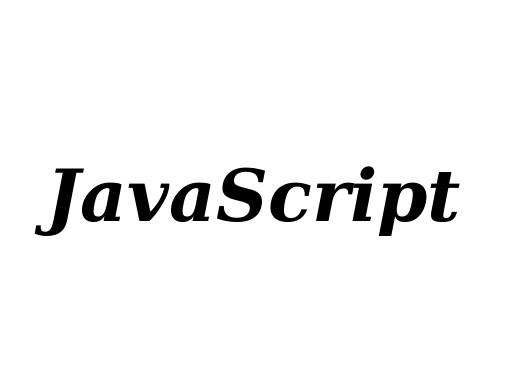
\includegraphics[width=.14\textwidth]{image/javascript-logo.png}
\end{wrapfigure}


JavaScript is a scripting language supported by all popular web browsers. Has extensive frameworks built around it and allows for rapid development. It is also possible to let the user write commands using JavaScript directly.

\subsubsection{Conclusion}
As a team, we have extensive experience with Java, and less with the other technologies. However, we all have at least some experience with JavaScript, and we believe that it is the better choice for this project: The DSL can be implemented by allowing the user to perform operations on the JavaScript objects using (a subset of) the JavaScript language itself. There are also excellent tools for transfer and storage of JavaScript objects. Furthermore, communication between JavaScript and HTML elements is easily achieved.

\subsubsection{JavaScript Related technologies}

\textbf{jQuery}\\*
A JavaScript library that simplifies how to use JavaScript to interact with the webpage, notably selection of Document Object Model elements.\\*
\\*
\textbf{MooTools}\\*
A JavaScript framework that, notably, enhances the Document Object Model and JavaScript's object oriented programming model.\\
\\*
\textbf{Dojo}\\*
A JavaScript toolkit offering asynchronous communication, a packaging system and systems for data storage. Intended to ease rapid JavaScript web development.\\*
\\*
\textbf{HTML5}\\*
A revision of the HTML standard currently still in development. Notably, it supplies support for multimedia and more advanced user interface elements. Is commonly used in conjunction with JavaScript.\\*
\\*
\textbf{CSS}\\*
Cascading Style Sheets, used to specify a consistent look and feel to a series of HTML documents.\\*


\subsection{Synchronization Technologies}
We will be adding a library for bi-directional real time communications between the server and the client, to easily detect changes in the objects on both sides and to replicate these changes to the other side lightning fast. This functionality will ensure data consistency between the client and server side. To make these updates fast and to avoid extra work in creating this functionality ourselves, we will employ an external library to get the work done.

\subsubsection{Pusher}

\begin{wrapfigure}{r}{.2\textwidth}
\centering

\includegraphics[width=.19\textwidth]{image/pusher-logo.jpg}
\end{wrapfigure}

Pusher is a cloud based system which offers a hosted API. It relies on the use of HTML5 WebSockets, which provides bi-directional communication over a TCP channel. It is a widely used solution which is well documented, and it support for a lot of libraries for both the server and client side. The web-site offers tutorials and extensive documentation on the most popular libraries. Pusher creates channels that can be both listened and published to. If multiple devices are connected to the same channel, they will receive any messages sent to the channel almost simultaneously. Pusher offers a free account(an account is needed to use the system) which offers all the basic functionality we need, with up to 20 connections and 3 million messages per month.
\begin{figure}
\centering
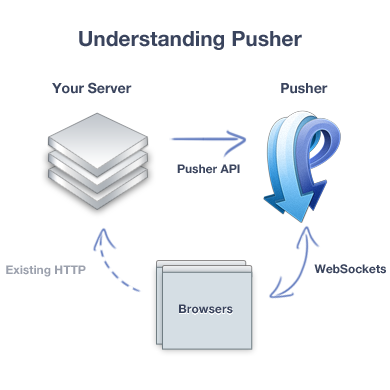
\includegraphics[width=3in]{image/pusher-explained.png}
\caption{Pusher Explained}
\end{figure}

\subsubsection{PubNub}

\begin{wrapfigure}{r}{.2\textwidth}
\centering

\includegraphics[width=.19\textwidth]{image/pubnub-logo.png}
\end{wrapfigure}

Like Pusher, PubNub is a push service hosted in the cloud. It is written entirely in C, which gives it extremely fast performance and enables it to push over 1 million messages a second. It offers great documentation and support for the most popular libraries on both the client and server side and its in widespread use. Like Pusher it relies on channels for communication which you can subscribe and publish to, and in essence the two solutions work in the same intuitive way. PubNub offers a free account with 1 million messages a month and up to 100 connections.

\subsubsection{Other Technologies}
We considered other similar alternatives as well, like Socket.io, Vert.x and Akka. But they either lacked support for the technologies we have chosen for the system, or lacked the extensive documentation and widespread use that Pusher and PubNub provides. We were also left with the impression that we would spend more time implementing these services than if we opted for either Pusher or PubNub.

\subsubsection{Conclusion}
Pusher and PubNub are both great systems that are widely used and they both offer extensive documentation. They cover the specific functionality we need for this project, which is to replicate the changes on both the client and server side. They both offer free accounts with more than enough connections and messages each month to cover our needs. So this decision will come down to our gut feeling. As none of the developers have any experience in using either system, the most important factor for this decision is that the system is well documented and easy to use. During research it became apparent that PubNub is the most widespread solution as of today. If we run into any problems implementing and using the system, it is likely someone has already provided a solution for it. So the decision ultimately fell on using PubNub.


\subsection{Markup Languages}
When communicating between the client and the server we need a data exchange format to represent objects and actions. The format has to be able to serialize and deserialize them on sending and receiving. The two alternatives most commonly in use today for solving this problem is XML (Extensive Markup Language) and JSON (JavaScript Object Notation).

\subsubsection{XML}
In widespread use in a lot of areas as of today and boasts great support and documentation. Originally meant to be a document markup language, but has over the years been used as a data representation language as well. It is suited to describe complex objects and documents, and it is easy to extend. Generally thought of as the more secure option of the two.

\subsubsection{JSON}
As the name suggest JSON is serialized JavaScript objects, well suited for web development, and very fast. JSON is easy for JavaScript to parse(we will be using JavaScript on both server and client), and the language has built in support for serializing and evaluating JSON data. Its small, simple, and easy to use. JSON is especially good at representing programming-language objects. It has gained a great deal of popularity in recent years, and it is well documented.

\subsubsection{Conclusion}
Both languages is well supported in almost all web related libraries, and they are both extensively documented. As security is not a main concern of this project, the fact that XML is more secure will not influence the decision. JSON will be used for this project. It covers the functionality we need, and it is generally thought of as the easier language to use. It is perfectly suited for web- development and JavaScript, which is the domain of this project. In addition the developers have more experience in using JSON than XML.

\section{Development Methodology}
\subsection{Agile vs Waterfall}
The waterfall method focus on planning the future in detail. It follows the principle of “Big Design Up Front”. It relies on the fact that you are able to report exactly what features that are going to be implemented and tasks are planned for the entire length of the project. It forces you to specify all the requirements early in the development, when you actually know the least about the project and the problems that are to be solved. The rationale behind this is that time spent early on making sure requirements and design are correct saves you much time and effort later. A development team using the waterfall method will only consider to implement the most valuable changes, as changes in this process are time consuming and often requires that completed work is started over. The method places a lot of emphasis on documentation. 

Agile methods, as opposed to the predictive methods, are designed to plan for changes in the requirements and features of a project. It emphasises on working code as primary measure of progress, instead of extensive documentation of for example the requirements. Agile methods consists of iterative and incremental steps in the development process, where requirements and solutions evolve through the course of the project. Requirements are bound to change, either because the customer didn't understand the problem in the beginning or because they would like to add new features. Agile methods facilitates the ability to accommodate these changes. Most agile methods includes delivering a working product in incremental stages, and gives the customer something to relate to during the developments process. The CHAOS Manifesto is a survey published by the Standish Group each year and it measures the success of IT- projects. It divides the projects into 3 groups; Success, meaning it completed on time and budget, with all features and functions as specified. Challenged, meaning it  completed, but was over cost, over time, and/or lacking all of the features and functions that were originally specified. Failed, meaning the project was abandoned or cancelled at some point and thus became a total loss. As Figure~\ref{figure:devchart} illustrates, agile methods although not perfect by any means, more often result in products that are successful(the method used for measuring the success of a project is to some degree debated, but the results serves a purpose nevertheless).

\begin{figure}
\centering
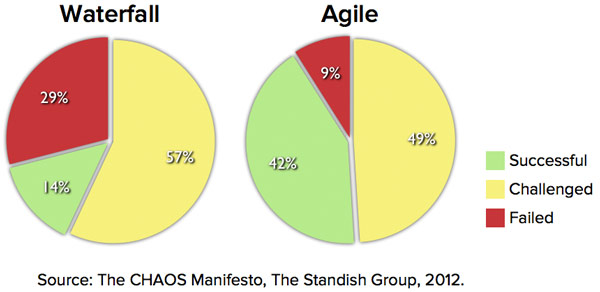
\includegraphics[width=3in]{image/Agile-Waterfall.jpeg}
\caption{Waterfall vs. Agile}
\label{figure:devchart}
\end{figure}

\subsection{Agile Methods}
There exists a lot agile methods for software development, and although all of them follow the basic principles of agile development, they differ in a lot of areas. Following is a detailed description of three different agile methods.

\subsubsection{Scrum}
Scrum is an iterative, incremental software development model with several short sprints - complete small sets of tasks each sprint.

\begin{figure}
\centering
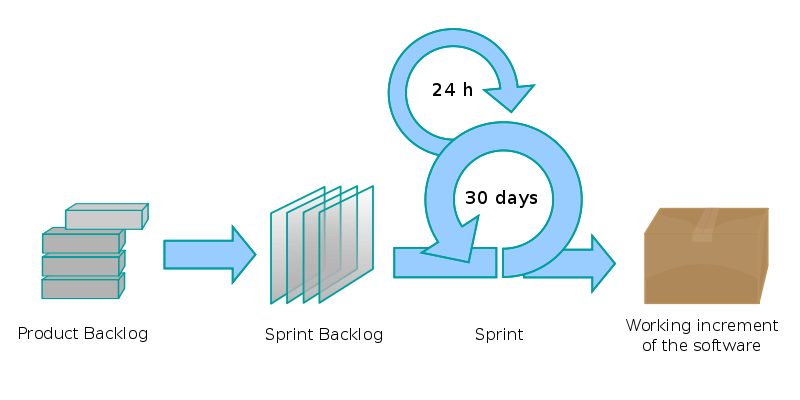
\includegraphics[width=4in]{image/Scrum_process.png}
\caption{Scrum Process}
\label{figure:scrumprocess}
\end{figure}


The Roles: 
\begin{itemize}

\item The Scrum master, who is responsible for leading the process and to enforce the Scrum rules onto the team. He has to make sure that the development team does not overestimate what they can handle during one sprint. He leads the scrum meetings and enlightens and handles obstacles that may appear. 

\item The product owner, represents the stakeholders and is the voice of the customer.

\item The development team, is responsible for delivering potentially shippable product increments at the end of each Sprint. A development team is made up of 3–9 people with cross-functional skills.

\end{itemize}

The Sprints:
\begin{itemize}

\item Normally last from 7 to 30 days .
\item Starts with a planning meeting, where tasks are identified and goals for the sprint is set.
\item Product owner tells the team what tasks should be done in the sprint.
\item The tasks comes from a prioritized list of requirements called the backlog.
\item The team determines what is possible based on this and records this in a sprint backlog.
\item The goals should not be changed during the sprint.

\end{itemize}

The Scrum process is well suited for projects where its difficult to plan too far ahead, where at least some of the aspects of the project are unknown. Its a versatile process which is gives you the ability to handle changes in the requirements and demands from the customer. It allows for the developers to work on different parts of the project at the same time. The design, requirements of the system are not set in stone from the start, and are allowed to evolve during the process. The process delivers unfinished versions at the end of each sprint, which gives the customer a chance to try the system and give continuous feedback to the developers. The Scrum process is somewhat complex, and it will take time to properly learn and execute the method. You also have to decide on what type of Scrum you are going to use, as there exists multiple forms of Scrum. This can prove to be a time consuming process. And even though the team members know Scrum, they will have to learn the version of scrum decided upon, if it turns out to differ from the one they are used to.
\footnote{\url{http://en.wikipedia.org/wiki/Scrum_(development)}}

\subsubsection{DSDM Atern}
DSDM(Dynamic System Development Method) is an agile software development method, and it was originally meant to provide some discipline to the Rapid Application Development method. The most recent version was launched in 2007 in an effort to make DSDM tool and technique independent, and its called Atern. DSDM is an iterative and incremental approach that embraces principles of agile development, including continuous user/customer involvement. It enforces you to deliver incremental versions of the product to the customer, where the main criteria of acceptance is that it meets the current business needs of the customer. It follows the principle that it is always better to deliver something “good enough” early than to deliver everything “perfect” in the end.

DSDM as a method fixes costs, quality and time at the beginning of the project. Through a prioritization method called the “MoSCoW Method”, with musts, shoulds, coulds and won’t haves, it adjusts the scope of the project to meet the given time frame. This allows the development team to focus on the critical functions of the system rather than delivering a perfect system. The method puts a strong focus on actively involving the customer in the development, and continually confirm the solution. The principle-list of DSDM is quite long and complex. For a team that is not experienced in using the method, the process of learning the method will be time consuming. Also, always having to display the progress to the customer can be time consuming and hinder the development effort. Testing is central and shall be done through the whole development process.
\footnote{\url{http://en.wikipedia.org/wiki/DSDM}}

\subsubsection{Extreme Programming}
Extreme programming, hereby referred to as XP, is an agile method designed to reduce cost of changes in requirements by having multiple short development cycles. It includes elements such as pair- programming, extensive code review and unit testing of all the elements of the code. It emphasises frequent communication with the customer and between the developers. The method embraces changes in the requirements of the project, and it doesn't attempt to define a stable set of requirements at the beginning of the project. In XP a representative for the customer is always available on site to answer any questions the developers might have. It also focuses on frequent releases of working code which serves as checkpoints where the customer can add new requirements. XP puts a lot of focus on the code of the project, the advocates of XP argues that the code is the only truly important product of the system development process. XP as a process does not produce a lot of written documents during the development of the project. In XP programmers are expected to assume a unified client viewpoint and focus on coding rather than documentation of compromise objectives and constraints.
\footnote{\url{http://en.wikipedia.org/wiki/Extreme_Programming}}

\subsection{Conclusion}
If all of the requirements of this project were known in advance and provided by the customer, or the features of the finished product was known and unlikely to change, the waterfall method might be the way to go. But this is a prototype, proof of concept type of project where very little is known about the final product. We were certainly not presented with a finished set of requirements at the beginning of the project, and the requirements we settle on before we start the implementation are also more than likely to change during development. These kind of changes in a waterfall process will be time consuming. Thats why we think that an agile development method will be the best choice for this project.

All of the agile methods described above exhibits properties that will come in useful in this project. They are all based on iterative and incremental development steps, delivering prototypes for the customer to test after each step. This will give the customer a chance to try out unfinished versions of the product and give continuous feedback throughout the project. It can also help the customer to identify new features that they would like to add. They also allows the customer to decide which features to implement in each step, ensuring that the final product will contain the features the customer really need. The agile methods embrace changes in the requirement and provides ways to handle those changes. They also encourage tight and continuous communication with the customer, which is important to be able to deliver a product that the customer is satisfied with. Of the three methods the group members are most familiar with the Scrum process. The DSDM method is complex and will take a considerable effort to learn and execute correctly. As none of the group members have used DSDM, and we have a limited amount of time in this project, DSDM is of the table. XP puts a lot of focus on the code, and delivers a minimal set of documents. We are to write an extensive report about the project, and document every part of it, including compromises and assumptions made. The amount of code in this project will be limited and none of the team members have any experience in working with XP. As a result, XP seems like a bad fit for our project. The Scrum process does not put as much focus on documentation as the waterfall process, but we think that the amount of documentation produced during the Scrum process will be satisfactory for the report. It will take time to learn how to execute Scrum properly, but since all of the group members are familiar with the basics of process, we think it won’t be too time consuming and worth the effort. The final decision then is to use Scrum as a development method for this project.

\section{Software Testing}

\subsection{Testing Methods}
The purpose of software testing is to uncover software bugs in the system and to document that the system meet the requirements and functionality that was agreed upon for the system. Testing can be implemented at any stage in the development process, traditionally it is performed after the requirements have been defined and the implementation is completed. In agile development processes however, the testing is an ongoing process. The chosen development methodology will in most cases govern the type of testing implemented in a given project.
\cite{sommerville2011software}

Software testing methods are traditionally divided into white- and black- box testing. They differ mainly in how the test engineer derives test cases.

\subsubsection{White- Box Testing}
White- box testing focus on the internal structures of a system, and it uses this internal perspective to derive test cases. White- box testing is usually done at unit level, testing specific parts or components of the code. This kind of testing focus on how something is implemented and not necessarily why. Unit testing alone cannot verify the functionality of a piece of software is supposed to exhibit. It can uncover many errors or problems, but it might not detect unimplemented parts of the specification or missing requirements.

\subsubsection{Black- Box Testing}
Black- box testing handles the software as a black- box, meaning it observes the functionality the system exhibits and not the specifics on how it is implemented. The tester only needs to be aware of what the program is supposed to do, he doesn't need to know the specifics on how the functionality is implemented in the code. Black- box testing is typically performed to check if the functionality of the program is according to the agreed upon requirements, both functional and nonfunctional. Black- box testing is usually done at the component, system and release levels of testing. The main advantage of black- box testing is that no programming knowledge is needed to actually perform the tests. This way you can hire someone outside the development team who has had nothing to do with the implementation of the code to write and perform the tests, and you achieve as little ownership of the code as possible. An argument can be made though that this lack of insight in the specifics of the source code will result in repeated testing of some parts of the code, while other parts could be left untested.

\subsubsection{Test Driven Development}
The principle behind TDD is to develop the code incrementally, along with test for that increment. You don’t move on until the code passes its test. The tests are to be written before you actually implement the new functionality. The process helps programmers clarify their ideas of what a code segment is actually supposed to do. The process is often used in agile development methods.
Benefits from TDD include: 
\begin{itemize}

\item Code coverage, every code segment should be covered at least one test.

\item Regression testing, check to see if changes in the code have not introduced new bugs.

\item Simplified debugging, when a test fails it should be obvious where the problem lies, no need for a debug tool.

\item System documentation, the tests themselves act as a form of documentation that describe what the code should be doing.

\end{itemize}

\cite{beck2003test-driven}

\subsubsection{Automated Tests}
Automated offers the ability to automatically do regression tests, i.e. testing to uncover if any new code has broken a test that previously passed. If we opt for manual testing regression testing will be very time consuming as every test done so far has to be done over again. With an automated testing framework this job will be a lot easier as you can run a great number of tests in a matter of seconds. Most development languages offers libraries for automated testing.


\subsection{Testing Levels}
Testing can be done at many different levels and in different stages in the development process. Following is the most common partitioning of testing levels and a description on each of them.

\subsubsection{Unit Testing}
Unit testing aims to check specific components, such as methods and objects. Typically you will be testing objects, and you should provide test coverage of all the features of that object. Its important to choose effective unit test cases, that reflect normal operation and they should show that the specific component works. Abnormal inputs should also be included to check if these are processed correctly.

\subsubsection{Component Testing}
Tests bigger components of the system, and their interfaces(communication with other components). Made up of several interacting objects. Component testing is mainly a tool to check if component interfaces behaves according to its specification.

\subsubsection{System Testing}
In a given development project there may be several reusable components that have been developed separately and COTS systems, that has to be integrated with newly developed components. The complete system composing of the different parts is tested at this level. Components developed by different team members or groups may also be integrated and tested at this stage.

\subsubsection{Release Testing}
Release testing is the process of testing a particular release of the system that is intended for use outside of the development team. Often a separate team that has not been involved in the development perform this testing. These kind of tests should focus on finding bugs in the complete system. The objective is to prove to the customer that the product is good enough. This kind of testing could either be based on the requirements of the system or on user scenarios.

\subsubsection{User Testing}
This is a stage in the testing process in which users or customers provide feedback and advice. This could be an informal process where end- users experiment with a new system too see if they like it and that it conforms to their specific needs. Testing on end- users is essential for achieving success in a software process as replicating the exact working environment the system will be used in is difficult to achieve during development. The end users can help provide feedback on how specific functionality will work in an actual work environment.

Another form of user testing involves the customer and its called acceptance testing. Its a process where the customer formally tests a system to decide whether or not it should be accepted, where acceptance implies that payment for the system should be made. Acceptance testing is performed after the release testing phase.

\subsection{Conclusion}
The concept of TDD is to develop exhaustive tests that specify the system, and then writing code with the goal of satisfying the tests. This is useful in systems where the key functionality is in the form of program logic that can be verified to conform to the specification. It is difficult to write such exhaustive tests in applications that rely heavily on GUIs, network connections and database systems because of the added complexity and heterogeneousness that these features involve. In addition, our prototype's exact specifications are likely to change during development, requiring large amounts of test rewriting in the case of TDD, because the tests will be more numerous and because the tests must be more strict. As a result we have opted not to use TDD in this project. We will however be utilizing unit tests with an automated testing framework where it is appropriate and will harvest some of the advantages linked to TDD, like the automated regression testing.

We will be writing unit tests throughout the implementation process and run these continuously. These tests will not be included in the report as test cases. The test cases will rather comprise of component and system tests. Component tests will be used to test specific components and their functionality as well as their interaction with other components. System tests will be used on the system as a whole to check if it meets the agreed upon requirements. These test cases will be derived from the requirements. We will also try include some acceptance tests to include the customer in the testing process. 

We will be utilizing user testing and involve end users to get feedback on the entire system or specific functions. This testing will mainly be used to get feedback on the domain scripting language and how easy it is to understand and use. Preferably it will be done continuously throughout the development process. It is important to involve users as the goal of this project is to ease their workflow. As we are not working with an existing system thats actually in use, there will not exist any real users of this system with experience using it. We will therefore mainly be using our fellow students as test subjects, as they are readily available and technically competent enough to understand the concept and act as superusers. In addition the customer has stated that it will encourage employees from the entire company to us give feedback if we ask for it. Specific solutions can be sent to the customer representative which in turn will relay it to experts on the area it concerns.


\section{Code conventions}
\subsection*{JSLint}
JSLint looks through JavaScript code and detects potentially problematic and unusual syntax in the code to improve the quality of the code. 

JavaScript was originally aimed for web pages with small tasks where the Java platform was too heavy to run and develop for. But JavaScript is capable of much more, and has became used in more and larger projects. However, the lenient and flexible syntax useful for small tasks has proven to make JavaScript troublesome for larger projects. JSLint helps the developer in handling this. \cite{jslint-about}

\subsection*{JSHint}
JSHint is a fork of JSLint which was designed with similar goals of enforcing code quality and avoiding common programming errors, but in a more lenient manner. JSLint is criticized for being a tool that is not first and foremost helpful in preventing bugs or improving readability, but rather a tool that enforces any strict convention as a goal in itself. JSHint attempts to alleviate this, and is more configurable and exhibits less absolutist behaviour. \cite{jshint-about}

\subsection*{Comparison and Conclusion}
We chose JSHint, this is why.
JSLint is a stricter version of JSHint. We started out with JSLint after we had written some lines of code, and saw that it produced closer to a 100 errors, and satisfying the linter would mean to rewrite most of the code. After this discovery we tested the JSHint fork of JSLint, which  “make a more configurable version of JSLint—the one that doesn't enforce one particular coding style on its users—” - \footnote{\url{http://www.jshint.com/about/}}. JSHint is also much more involved in the JavaScript developer community, and based on this. JSHint did not produce as many errors, and did not require as much effort to satisfy.
JSLint enforces its own way of coding, which is not always what you want from a linter. The team switches between different coding languages both inside and outside the project. It is unnecessarily time consuming to get into the mind of Douglas Crockford (maker of JSLint) every time you switch to JavaScript. JavaScript is a dynamic language which lets you write the same code in so many different ways, and the way of JSLint isn’t always the way.
\footnote{\url{http://www.jslint.com/}}
\footnote{\url{http://www.jshint.com/}}

\section{Version Control}
\subsection{Git}
Git is a open source project for distribution and version control of source code. Linus Torvalds wanted a source code manager with emphasis on speed, and git was the product of this. Git has the features show in table \ref{table-gitfeatures}.

\begin{table}
\centering
\begin{tabularx}{\textwidth}{ l X l }
  \textbf{Feature}      & \textbf{Description} \\
  \hline \\ [-1.5ex]
  Branching and merging & Through this the developer can have multiple branches of the system, which can be independent of each other, which makes rollbacks, merging and editing simple and efficient. \vspace*{0.7ex} \\
  \hline \\ [-1.5ex]
  Small and fast        & Operations are made locally, which makes more efficient than other similar systems such as SVN. \\
  \hline \\ [-1.5ex]
  Distributed           & The distribution works through cloning of the working repository, this means that every user has a backup of the system in case of a crash. The distributed code can be pushed back to the shared repository with changes, and will update the system for other users to fetch back to their own clone. \\
  \hline \\ [-1.5ex]
  Data assurance        & The files and commits in the repositories has its own checksum, and can be retrieved through this checksum, this assures that a user cannot fetch anything out of the repository other than what has been put in. \\
  \hline \\ [-1.5ex]
  Staging area          & Before completing a commit, there is possible to review the changes. This makes it possible to decide upon which files to commit, if not all changes are to be pushed to the main repository. \\
  \hline \\ [-1.5ex]
  Free and open source  & The user are free to inspect the source code or contribute to the project. Git is under the GPLv2 software license\\
\end{tabularx}
\caption{Git features}
\label{table-gitfeatures}
\end{table}

%[https://git.wiki.kernel.org/index.php/Main_Page][http://git-scm.com/]

\subsection{Subversion}
Apache Subversion (SVN) is open source. It is a cross-platform version control tool, used mainly for sharing source code, web pages and documentation. SVN is designed to be central, where you commit to one server. Some of SVN's features are shown in table \ref{table-subversionfeatures}.

\begin{table}
\centering
\begin{tabularx}{\textwidth}{ l X l }
  \textbf{Feature}      & \textbf{Description} \\
  \hline \\ [-1.5ex]
  Branching and tagging are cheap   & This can be done in constant time \vspace*{0.7ex} \\
  \hline \\ [-1.5ex]
  Merge tracking                    & SVN lets the user track the changes between lines of development \\
  \hline \\ [-1.5ex]
  Standalone server option          & The standalon option lets the user run their own server, other then an apached HTTPD server \\
  \hline \\ [-1.5ex]
  Interactive conflict resolution   & Merging conflictsis made easy through either graphical user interface of the commandline. \\
  \hline \\ [-1.5ex]
  Atomic commits                    & There is no part of the file will be commited if not the whole file is commited. \\
  \hline \\ [-1.5ex]
  Free and open source              & The user are free to inspect the source code or contribute to the project. SVN is under the Apache License \\
\end{tabularx}
\caption{Subversion features}
\label{table-subversionfeatures}
\end{table}

%http://subversion.apache.org/

\subsection{Conclusion}
Most of the team is fearly familliar with the Git version control tool. It is important that it is not centrelised like the Subversion tool, git aloves the members to easy work offline, since git lets the user always be "online" through their own cloned repository.
The git version control tool also alos the team to disribute the reportfiles, images and database-files more easily since git is a "file contetn managment tool". 
The Git repository is easy to distribute of use through GitHub \ref{GitHub}, and makes the project reachable for all the team members.
The mentioned points and the fact that the team is more familiar with Git then SVN made us choose Git as our version control system.
